\begin{thesischapter}{2} {Análisis, diseño e implementación del Juego Serio}
    En este capítulo se discuten los detalles de desarrollo de los aspectos citados en el capítulo anterior. Este comienza con una descripción y caracterización general del sistema, donde se  abordan cada uno de los componentes requeridos para su completo funcionamiento. Posteriormente se detallan la ingienría de software requerida en la etapa de conceptualización de la aplicación, se explica de forma 
    detallada los aspectos teóricos y de implementación de la base de datos, el funcionamiento del protocolo de comunicación y por último los escenarios de juegos requeridos en las rutinas de entrenamiento ligero y clínico, y las estadísticas generadas por estos. Como herramienta de desarrollo se utilizó c\#.

    \subthesischapter{Descripción y caracterización del sistema}
    Antes de adentrarnos en los aspectos técnicos de la ingeniería de software, es esencial comprender el contexto en 
    el que se desarrolla la aplicación. En nuestro caso, se trata de un sistema de rehabilitación neuromuscular lógicamente 
    separado por 2 componentes autónomos que interactúan entre si: juego serio y pedal motorizado. 

    \vspace{10pt} % Descripción del sistema 
    En la figura \ref{fig: sa} se presenta el \textbf{sistema de adquisición de datos}\footnote{Hace refenrencia al pedal motorizado}, en esta se puede observar la ubicación de los sensores MyoWare  utilizado para la medición de la activación muscular a través del potencial eléctrico, conocida como electromiografía y un sensor óptico SHARP modelo GP1A51HRJ00F con salida  \textbf{OPIC}\footnote{Circuito integrado fotoacoplador de salida} ubicado en la biela del pedal el cual es utilizado para la obtención de la velocidad angular. Adicionalmente el sistema utiliza un microcontrolador Arduino DUE encargado de coordinar y controlar las operaciones de adquisición de datos. Su función principal es gestionar la comunicación entre los sensores de adquisición de datos y el resto del sistema.

    \begin{figure}[ht]
        \centering
        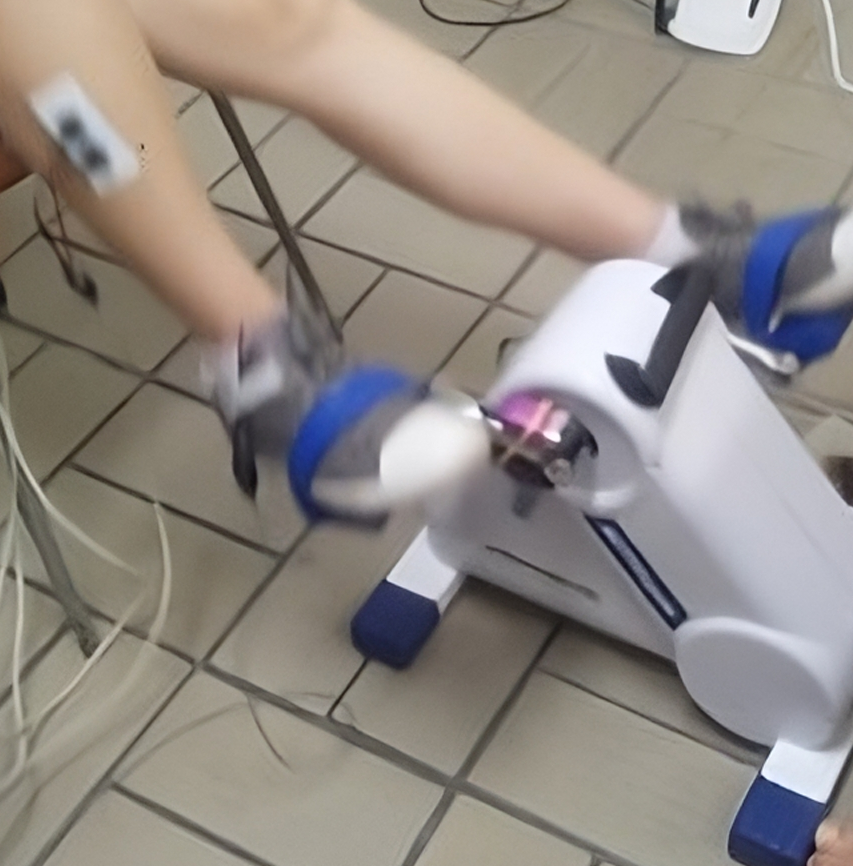
\includegraphics[scale=0.2]{images/sa.png}
        \caption{Sistema de adquisición de datos}
        \label{fig: sa}
    \end{figure}    

    \vspace{10pt} % Funciones de los componentes 
    El funcionamiento del videojuego se logra por medio de dos componentes del pedal:
    \begin{itemize}
        \item El primer componente (sensor óptico) controla la velocidad de movimiento en el videojuego, por
        medio de la acción de pedaleo del paciente en rehabilitación. A medida
        que se logra una velocidad definida, se envía la orden de movimiento al videojuego y 
        este responde con el movimiento del avatar en la escena, el cual se encuentra en una pista 
        cuyo objetivo será alcanzar los mejores resultados de tiempo, distancia o  MCV(Máxima contracción voluntaria).
        \item El segundo componente del sistema (sensores de EMG) tienen la función de capturar la señal EMG obtenida en la 
        una rutina de entrenamiento y ser usados tanto en la dificultad de los niveles de entrenamiento de la rutina clínica como para la 
        estadística de la misma.
    \end{itemize}
    
    
    Dichos componentes tanto internos como externos se encuentran orientados hacia 
    la realización de un objetivo común, el desarrollo de la capcidad física tanto para usuarios 
    sanos como enfermos. A continuación se presentan las características funcionales 
    del sistema, ver figura~\ref{fig: system}:

    \vspace{10pt}
    La aplicación de juego serio es responsable de:
    \begin{itemize}
        \item Recibir y procesar las señales de la plataforma Arduino incluido en el pedal para ser utilizadas tanto en la 
              animación de la escena como en la estadística .
        \item La carga y procesamiento de las escenas y los paradigmas de las rutinas junto a la lógica asociada. 
        \item Procesar los eventos registrados durante la realización de la rutina y devolver un análisis sobre los resultados.
        \item Gestionar los datos del usuario.
    \end{itemize}

    \vspace{10pt}
    El pedal motorizado es responsable de:
    \begin{itemize}
        \item Registrar a partir de electrodos las señales EMG del cuerpo humano correspondientes al tren inferior.
        \item Registrar la velocidad angular en los pedales.
        \item Enviar en tiempo real los datos registrados a cualquier aplicación de juego serio sincronizada.
    \end{itemize}
    
    \begin{figure}[ht]
        \centering
        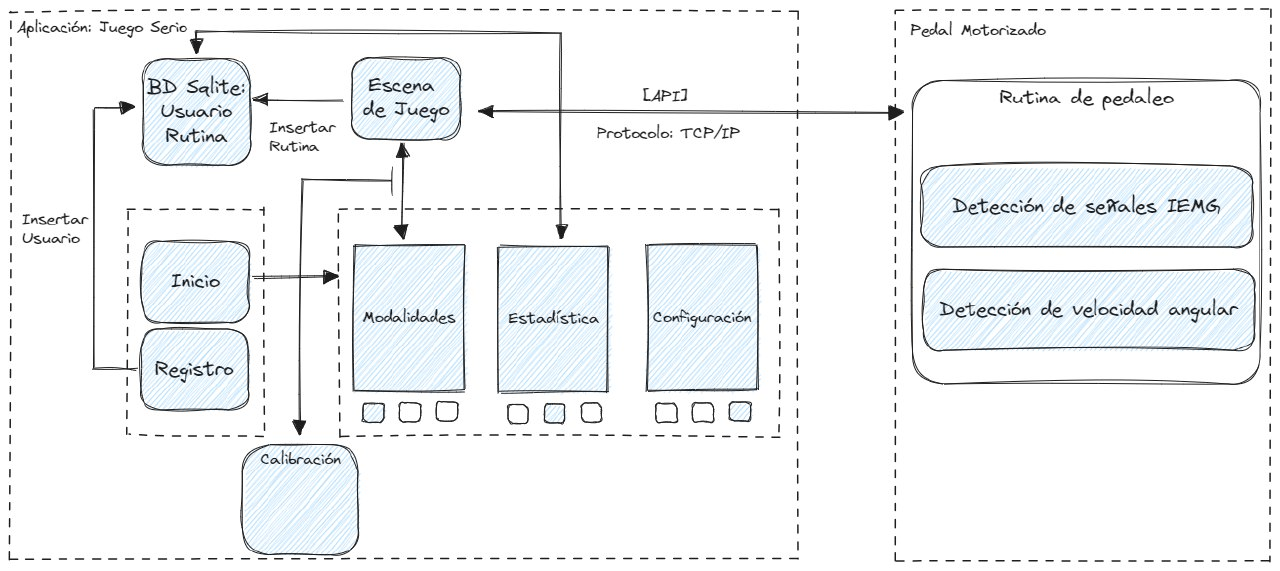
\includegraphics[scale=0.38]{images/system.jpg}
        \caption{Diagrama del sistema}
        \label{fig: system}
    \end{figure} 
    
    %--------------------------------------------
    \subthesischapter{Requisitos del Juego Serio}
    Un requisito es una restricción que el sistema debe cumplir. Tiene como propósito expresar un comportamiento o propiedad que 
    el sistema debe poseer~\cite{jacobson2000uml}. El objetivo esencial de un requisito es el de definir un comportamiento específico 
    de manera clara y comprensible. Pueden clasificarse en funcionales 
    y no funcionales.

    \subsubthesischapter{Requisitos funcionales}
    La integración de tecnologías de pedaleo en el campo de la rehabilitación neuromuscular ha abierto nuevas oportunidades 
    para mejorar la calidad y eficacia de las terapias. En particular, los juegos serios han demostrado ser una herramienta 
    efectiva para motivar a los pacientes durante el proceso de rehabilitación. Tomando como punto de partida lo anteriormente 
    abordado se hace necesario el desarrollo de una aplicación android que cumpliera con los siguientes requerimientos funcionales:    

    \begin{enumerate}
        \item Iniciar sesión en el sistema
        \item Registrarse en el sistema
        \item Eliminar cuenta de usuario
        \item Editar los datos del usuario
        \item Cerrar sesión en el sistema
        \item Enviar datos al pedal
        \item Recibir datos del pedal
        \item Establecer comunicación con el pedal
        \item Finalizar comunicación con el pedal
        \item Iniciar rutina
        \item Pausar o reanudar el rutina
        \item Finalizar rutina
        \item Mostrar estadísticas rutina
        \item Configurar rutina
        \item Iniciar calibración
        \item Guardar registro de comportamieto en archivo \textbf{logs}\footnote{Archivo de texto en el que constan cronológicamente los acontecimientos que han ido afectando a un sistema informático}
    \end{enumerate}
    \subsubthesischapter{Requisitos no funcionales}
    Los requisitos no funcionales son propiedades o cualidades que el producto debe tener. Enuncian los requisitos del sistema que no pueden ser expresados como funcionalidades en respuesta a alguna acción de un usuario. 
    En nuestro caso se identificaron los siguientes requisitos no funcionales:
        
    \begin{itemize}
        \item \underline{Requisitos de usabilidad}: La interfaz de trabajo del usuario con la herramienta deberá ser simple, interactiva e intuitiva y deberá notificar los diferentes errores que se produzcan durante su ejecución.
        \item \underline{Requisitos de escalabilidad}: La aplicación debería ser capaz de escalar para manejar un aumento en el número de usuarios o la cantidad de datos sin perder rendimiento.     
        \item \underline{Interoperabilidad}: Si la aplicación interactúa con otros sistemas, debe ser capaz de hacerlo de manera eficiente y sin problemas 
    \end{itemize}

    \newpage
    \subthesischapter{Definición de los casos de uso}
    \subsubthesischapter{Identificación de los actores}
    Los actores no son parte del sistema, pero sí pueden intercambiar información con él, ellos representan un rol que juegan una o varias personas, un equipo o un sistema automatizado. En la aplicación
    de juego serio se identificaron los siguientes actores:

    \begin{table}[ht]
        \centering
        \begin{tabularx}{\textwidth}{|l|X|}
            \hline
            \textbf{Actores} & \textbf{Descripción} \\\hline
            Usuario & Individuo que interactúa con el sistema para hacer uso de una rutina de entrenamiento
            como medio de rehabilitación, diversión o entrenamiento físico \\\hline
            Sistema & Es la misma aplicación que en determinadas ocasiones ejecuta funcionalidades automáticamente producto de la interacción con el pedal motorizado. \\\hline
        \end{tabularx}
        \label{tab: actores}
        \caption{Descripción de actores}
    \end{table}

    \subsubthesischapter{Identificación de los casos de usos}    
    Cada forma en que los actores usan el sistema se representa con un caso de 
    uso, como fragmentos de funcionalidad que el sistema ofrece para aportar solución a la necesidad de esta aplicación. 
    Los casos de uso que se definen para el sistema propuesto están reflejados en la cuadro: 3 con su respectivo diagrama
    en la figura: \ref{fig: use-cases-user}, \ref{fig: use-cases-system}:

    \begin{table}[h]
        \centering
        \begin{tabularx}{\textwidth}{|c|X|c|}
            \hline
            \textbf{Casos de uso} & \textbf{Descripción} & \textbf{Requisitos}\\\hline
            Iniciar sesión & Permite al usuario acceder al sistema & RF1\\\hline
            Registrar usuario & Permite guardar los datos de un usuario en la Base de Datos & RF2\\\hline
            Eliminar usuario & Permite eliminar la cuenta de un usuario en la Base de Datos & RF3\\\hline
            Editar datos del usuario & Permite actualizar losdatos personales del usuario en la Base de Datos & RF4\\\hline
            Cerrar sesión & Permite al usuario cerrar sesión en el sistema & RF5\\\hline
            Enviar datos al pedal & Permite a la aplicación enviar datos al pedal & RF6 \\\hline
            Recibir datos del pedal & Permite a la aplicación recibir los datos provenientes del pedal & RF7\\\hline
            Establecer comunicación & Permite establecer comunicación entre el dispositivo Android y el Pedal Motorizado & RF8\\\hline
            Finalizar Comunicación & Permite finalizar comunicación entre el dispositivo Android y el Pedal Motorizado & RF9\\\hline
            Iniciar rutina & Permite dar inicio a la rutina de entrenamiento & RF10\\\hline
            Pausar/Reanudar rutina & Permite pausar la etapa actual de la rutina & RF11\\\hline
            Finalizar rutina & Permite dar fin a la rutina de entrenamiento & RF12\\\hline
            Mostrar estadística & Permite mostrar estadísticas de las rutinas de entrenamiento  al usuario& RF13\\\hline
            Configurar rutina & Permite elegir la modalidad e insertar los parámetros de la rutina  & RF14\\\hline
            Iniciar calibración & Permite iniciar la calibración para la modalidad clínica  & RF15\\\hline
            Guardar logs & Permite almacenar los hechos ocurridos en el sistema en ficheros de logs & RF16\\\hline
            %Iniciar juego rutina libre & Permite dar inicio a la rutina de entrenamiento libre \\\hline
            %Iniciar juego rutina resistido & Permite dar inicio a la rutina de entrenamiento resistido \\\hline
        \end{tabularx}
        \label{tab: rf}
        \caption{Casos de uso del sistema}
    \end{table}
    
    \vspace*{50pt}
    \begin{figure}[h]
        \centering
        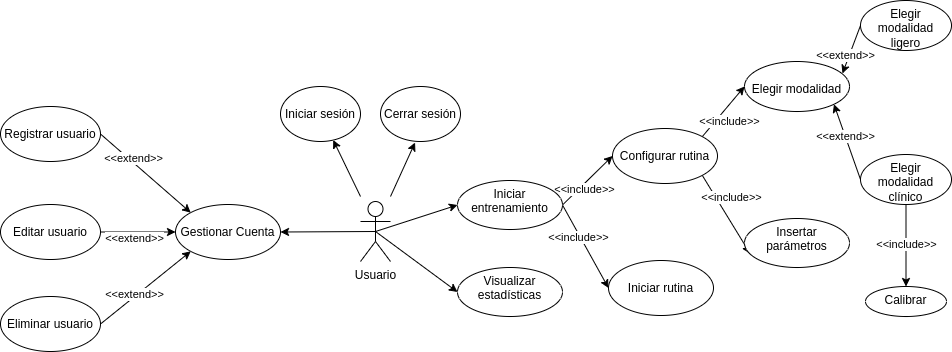
\includegraphics[scale=0.44]{images/diagram-usecase-user.png}
        \caption{Diagrama de casos de uso, actor usuario}
        \label{fig: use-cases-user}
    \end{figure}

    \vspace*{50pt}
    \begin{figure}[h]
        \centering
        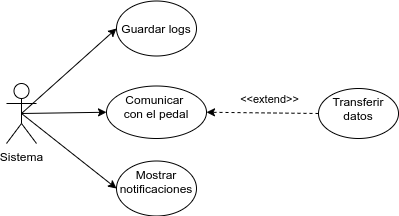
\includegraphics[scale=0.44]{images/diagram-usecase-system.png}
        \caption{Diagrama de Casos de Uso, actor sistema}
        \label{fig: use-cases-system}
    \end{figure}

    \vspace*{100pt}
    \subthesischapter{Realización de los casos de uso}
    La realización de los casos de uso en el análisis es una colaboración que describe cómo se lleva a cabo y ejecuta un caso de uso 
    determinado en término de las clases del análisis y de sus objetos en interacción, por lo tanto, se centra en los requisitos funcionales. 
    A continuación se describe el caso de uso de mayor relevancia.
    
    \begin{center}
        \begin{table}
            \begin{tabularx}{\textwidth}{|X|X|}
                \hline
                \textbf{Caso de uso:} & Entrenamiento \\\hline
                \textbf{Actores:}     & Usuario \\\hline
                
                \multicolumn{2}{|X|}{        
                \begin{minipage}[t]{0.925\columnwidth}
                    \textbf{Descripción:} \\
                    Permite iniciar una rutina de entrenamiento seleccionando entre las modalidades disponibles en el sistema
                    \vspace{2pt}
                \end{minipage}} \\\hline
                
                \textbf{Requisitos funcionales asociados:} &  RF10, RF14\\\hline
                \textbf{Precondiciones:} & \begin{itemize}
                                                \item Haber iniciado sesión en el sistema
                                                \item El módulo de comunicación del dispositivo móvil debe estar activado y conectado a la red wifi del pedal
                                                \end{itemize}\\\hline
                \textbf{Poscondiciones:} & Los resultados de la nueva rutina quedarán registrados en el sistema \\\hline
                
                % SECTION 1
                \multicolumn{2}{|X|}{        
                \begin{minipage}[t]{0.925\columnwidth}
                    \begin{center}
                        \textbf{Sección principal}
                    \end{center}
                \end{minipage}} \\\hline
                
                Acción del actor & Acción del sistema \\\hline
                1. El usuario selecciona la opción de entrenamiento en la vista principal, ver anexo 3. & 2. El sistema muestra la interfaz para la selección de la modalidad. \\\hline
                3. El especialista selecciona la opción que desea:
                \begin{itemize}
                    \item Caso <<Modalidad ligero>>: ir al curso alterno <<Modalidad ligero>>
                    \item Caso <<Modalidad clínico>>: ir al curso alterno <<Modalidad clínico>>
                \end{itemize} &  \\\hline
                
                % SECTION 2
                \multicolumn{2}{|X|}{        
                \begin{minipage}[t]{0.925\columnwidth}
                    \begin{center}
                        \textbf{Sección de cursos alternos}
                    \end{center}
                \end{minipage}} \\\hline
                \multicolumn{2}{|X|}{        
                \begin{minipage}[t]{0.925\columnwidth}
                        \textbf{Curso alterno: Modalidad ligero}
                \end{minipage}} \\\hline
                
                Acción del actor & Acción del sistema \\\hline
             
                & 
                1. El sistema construye la interfaz con los parámetros generales de la modalidad seleccionada, ver anexo 3 a). \\\hline
                2. El usuario inserta los valores de distancia y tiempo según la dificultad del entrenamiento que desee y presiona en el botón comenzar fig \ref{}. 
                & 
                3. El sistema muestra la escena de juego correspondiente a la modalidad elegida fig\ref{}. \\ &4. Termina el CU. \\\hline
                
                \multicolumn{2}{|X|}{        
                \begin{minipage}[t]{0.925\columnwidth}
                        \textbf{Curso alterno: Modalidad clínico}
                \end{minipage}} \\\hline
                
                Acción del actor & Acción del sistema \\\hline
                 
                & 
                1. El sistema construye la interfaz correspondiente a la sección de calibración, ver anexo 3 c). \\\hline
                \begin{enumerate}
                    \item[2.] El usuario presiona en los botones iniciar medición, calcular línea base y calcular MCV siguiendo el protocol médico de calibración.
                    \item[3.] El usuario presiona en el botón de modalidad clínico.
                \end{enumerate}
                &
                5. El sistema construye la interfaz con los parámetros generales de la modalidad seleccionada, ver anexo 3 b). \\\hline
                6. El usuario inserta los valores de distancia, tiempo y porciento de MCV según la dificultad del entrenamiento que desee y la calibración obtenida y luego presiona en el botón comenzar. 
                & 
                7. El sistema muestra la escena de juego correspondiente a la modalidad elegida fig\ref{}. \\ &4. Termina el CU. \\\hline
                

                %% ------------------------
                % \multicolumn{2}{|X|}{        
                % \begin{minipage}[t]{0.925\columnwidth}
                %     \begin{center}
                %         \textbf{Prototipo de UI}
                %     \end{center}                    
                % \end{minipage}} \\\hline
                
                % \multicolumn{2}{|X|}{        
                % \begin{minipage}[t]{0.925\columnwidth}
                %     \vspace{5pt}
                %     \begin{minipage}[t]{0.5\columnwidth}
                %         \centering
                %         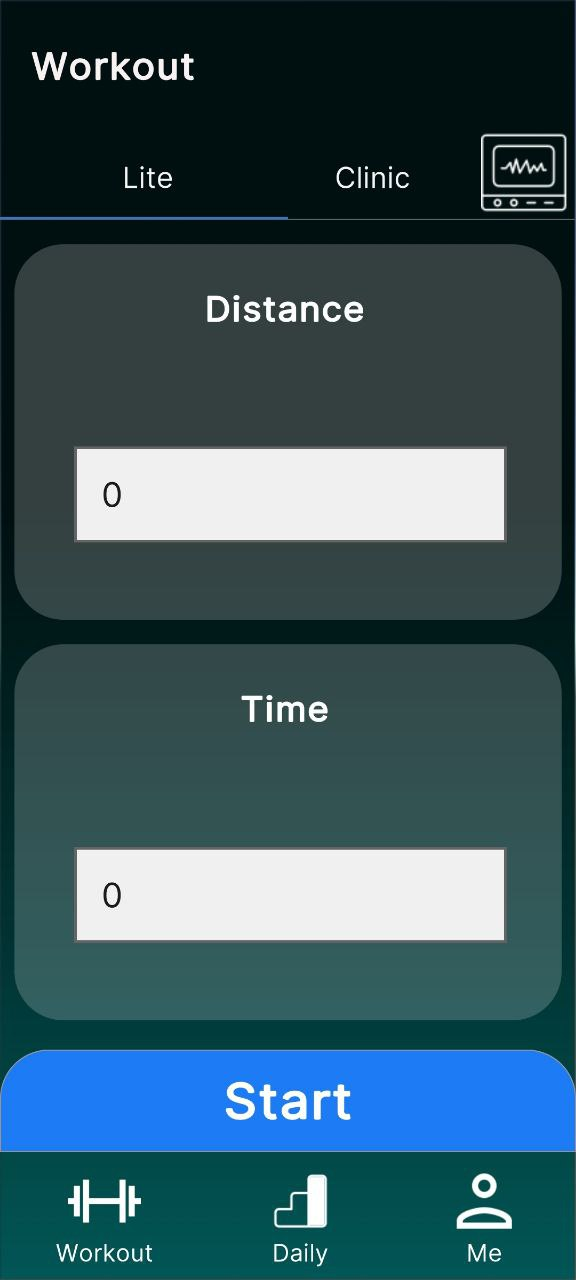
\includegraphics[scale=0.2]{images/ui/2.jpg}
                %         \caption{Pantalla principal}
                %         \label{display: 1}
                %     \end{minipage}
                % \end{minipage}} \\\hline
                


            \end{tabularx}

            \caption{Descripción del CU: Establecer comunicación con el pedal}
        \end{table}
    \end{center}
    
    % DATABASE --------------------------------------
    \newpage
    \subthesischapter{Diseño de la base de datos}
    Existen dos tipos prominentes de sistemas de gestión de bases de datos ampliamente reconocidos: uno conocido 
    como Lenguaje de Consulta Estructurado (SQL, por sus siglas en inglés) organiza los datos en estructuras tabulares, 
    mientras que el otro, denominado No-SQL, prescinde de las tablas y opta por almacenar datos en forma de objetos. 
    Contrariamente a SQL, el enfoque No-SQL no sigue una estructura rígida, permitiendo mayor flexibilidad en la 
    organización de los datos. No obstante, se ha observado que los sistemas No-SQL tienden a requerir una mayor 
    cantidad de recursos computacionales en comparación con las implementaciones SQL. En el contexto de aplicaciones 
    móviles, se ha preferido el uso de SQL debido a su eficiencia y menor consumo de recursos, lo que contribuye a una 
    experiencia de usuario más fluida y eficaz.

    \vspace{10pt}
    \subthesischapter{Modelo lógico}
    La descripción que surge de esta fase de diseño sirve como base para especificar la estructura conceptual de la base de datos. 
    La siguiente lista describe los principales requisitos para el registro de datos en el sistema:
    \begin{itemize}
        \item Los usuarios son reconocidos a través de un identificador único. En el sistema, se almacenan los detalles de identificación del usuario, los cuales se especifican en los requisitos de registro e incluyen el nombre completo del usuario, su dirección de correo electrónico y una contraseña asociada.
        \item Cada usuario tiene la capacidad de establecer múltiples rutinas de entrenamiento personalizadas. Estas rutinas están compuestas por un identificador exclusivo, el tipo de ejercicio elegido y los parámetros específicos que han sido configurados por el usuario. 
        \item Luego de terminada una rutina se almacena en el sistema los resultados obtenidos y la fecha de ejecución. 
    \end{itemize}   
    
    \vspace{10pt}
    \textbf{Designación de los conjuntos de entidades y de relaciones}\\
    Desde la especificación listada anteriormente se comienzan a
    identificar los conjuntos de entidades y relaciones, así como sus atributos:
    \begin{itemize}
        \item La entidad \underline{usuario}, con los atributos id\_usuario, nombre, correo, contraseña.
        \item La entidad \underline{rutina} con los atributos id\_rutina, modalidad, distancia, tiempo, \textbf{mcv\textsubscript{1}, mcv\textsubscript{2}, mcv\textsubscript{3}, mcv\textsubscript{4}}\footnote{mcv\textsubscript{i}: Valor porcentual definido de MCV en el canal i luego de la etapa de calibración}.
        \item La relación muchos a muchos de \underline{usuario} a \underline{rutinas} denominado \underline{ejecuta}, es decir un usuario puede ejecutar 
        varias rutinas y la misma rutina puede ser ejecutada por distintos usuarios. Dicha relación cuenta con los atributos id\_usuario, id\_rutina, resultados y fecha\_de\_ejecución. 
    \end{itemize}
    
    \vspace{10pt}
    El Diagrama de Entidad-Relación (E-R) que resulta de tales especificaciones para la descripción de los datos del sistema se presenta en la figura \ref{fig: diagram-er}.
    \begin{figure}[ht]
        \centering
        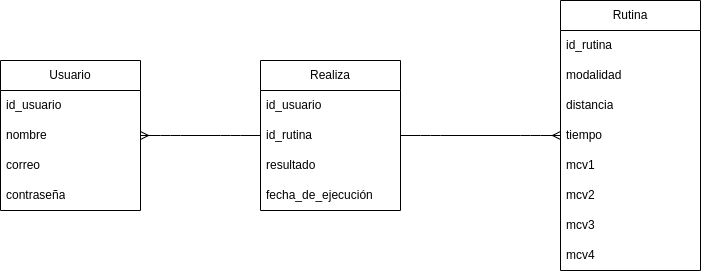
\includegraphics[scale=0.45]{images/diagram-er.png}
        \caption{Diagrama Entidad Relación}
        \label{fig: diagram-er}
    \end{figure}

    \subthesischapter{Modelo físico}
    El modelo físico de la base de datos consta de tres tablas principales: USER, RUTINE y DO en las que se han definido las siguientes 
    restricciones para mantener la integridad de los datos:

    \vspace{10pt}
    \begin{itemize}
        \item En la tabla USER, se ha establecido un campo ID como clave primaria, que se genera automáticamente mediante autoincremento 
        cada vez que se inserta una nueva fila. Los campos FULLNAME, EMAIL y PASSWORD almacenan la información del usuario.
    
        \item La tabla RUTINE contiene información sobre las rutinas de ejercicios. Se ha definido un campo ID como clave primaria con 
        autoincremento. Los campos MODALITY, TIME, DISTANCE, MCV0, MCV1, MCV2 y MCV3 almacenan los detalles de la rutina.
    
        \item En la tabla DO, se ha establecido un campo ID como clave primaria con autoincremento. Los campos ID\_MODALITY y ID\_USER actúan 
        como claves foráneas, haciendo referencia a las tablas RUTINE y USER respectivamente. El campo RESULT almacena los resultados obtenidos, 
        y el campo DATE registra la fecha de la realización de la rutina.
        
    \end{itemize}

    El esquema de las tablas de la base de datos, junto con las dependencias de clave primaria y las foráneas, se puede visualizar en la siguiente 
    porción de código:

\begin{center}
\begin{minipage}{0.8\textwidth}
\begin{lstlisting}[language=c,caption={Sección de código, constructor de la clase CibiofibDb}, label={code: database-code}]
public CibiofibDb() : base()
{
    IDbCommand dbcmd = getDbCommand();
    dbcmd.CommandText = "CREATE TABLE IF NOT EXISTS USER ( " +
                        "ID  INTEGER PRIMARY KEY AUTOINCREMENT, " +
                        "FULLNAME TEXT, " +
                        "EMAIL TEXT, " +
                        "PASSWORD TEXT )";
    dbcmd.ExecuteNonQuery();

    dbcmd = getDbCommand();
    dbcmd.CommandText = "CREATE TABLE IF NOT EXISTS RUTINE ( " +
                        "ID  INTEGER PRIMARY KEY AUTOINCREMENT, " +
                        "MODALITY INTEGER, " +
                        "TIME REAL, " +
                        "DISTANCE REAL, " +
                        "MCV0 REAL, " +
                        "MCV1 REAL, " +
                        "MCV2 REAL, " +
                        "MCV3 REAL )";

    dbcmd.ExecuteNonQuery();

    dbcmd = getDbCommand();
    dbcmd.CommandText = "CREATE TABLE IF NOT EXISTS DO ( " +
                    "ID  INTEGER PRIMARY KEY AUTOINCREMENT, " +
                    "USER_ID INTEGER, " +
                    "RUTINE_ID INTEGER, " +
                    "RESULT REAL, " +
                    "DATE TEXT, " +
    "FOREIGN KEY(USER_ID) REFERENCES USER(ID), " +
    "FOREIGN KEY(RUTINE_ID) REFERENCES RUTINE(ID))";

    dbcmd.ExecuteNonQuery();
}
\end{lstlisting}
\end{minipage}
\end{center}
    
\subthesischapter{Manipulación de los datos}
\vspace{10pt}
SQLite ha sido favorecido por los desarrolladores móviles y recomendado por la documentación oficial de Android. Aún  
Unity no ha brindado soporte oficial para crear bases de datos. Sin embargo, hemos ideado una manera de utilizar las 
ventajas de SQLite para nuestra aplicación. 

\vspace{10pt}
La idea utilizada fue agrupar los métodos y variables comunes en una clase. Luego extender la clase usando herencia para 
crear implementaciones reales. Fue creada una clase de alto nivel \underline{DataBaseModel} que se puede extender a otras clases, con el 
fin de acceder a las operaciones básicas de cualquier base de datos. Llamamos a estas operaciones básicas CURD: Crear, 
Actualizar, Leer y Borrar, ver figura \ref{fig: diagram-db}.
\begin{figure}[ht]
    \centering
    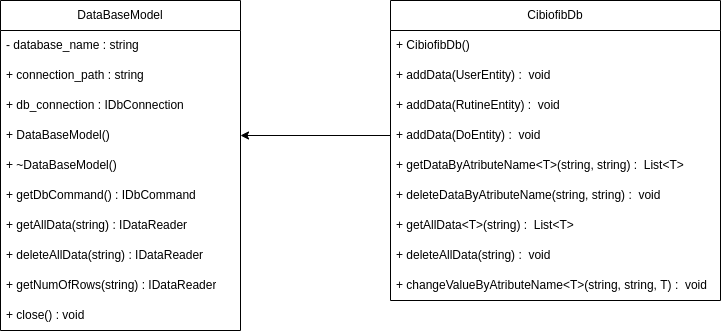
\includegraphics[scale=0.5]{images/diagram-db.png}
    \caption{Diagrama de clases}
    \label{fig: diagram-db}
\end{figure}

Para gestionar la información almacenada en la base de datos del sistema, se ha implementado un conjunto de funciones en C\# utilizando la biblioteca 
System.Data.SQLite. Estas funciones permiten realizar las operaciones CURD sobre las tablas USER, RUTINE y DO.


\subsubthesischapter{Conexión con la base de datos}
Para establecer la conexión con la base de datos, se utiliza la función getDbCommand() que devuelve un objeto de tipo IDbCommand. Este objeto se utiliza para ejecutar las instrucciones SQL en 
la base de datos. Se asegura que la conexión esté establecida correctamente antes de realizar cualquier operación de manipulación de datos.

\subsubthesischapter{Inserción en la base de datos}
Para insertar nuevos registros en las tablas USER, RUTINE o DO, se han implementado las funciones addData(UserEntity user), addData(RutineEntity rutine) y addData(DoEntity \_do) respectivamente. 
Estas funciones generan y ejecutan instrucciones SQL del tipo INSERT INTO para agregar nuevos registros a las tablas. Los datos son obtenidos de objetos de las clases UserEntity, RutineEntity y DoEntity
definidas en Models.cs.

\subsubthesischapter{Obtención de datos}
Para obtener datos de la base de datos, se han implementado las funciones getDataByAtributeName<T>(string atribute, string name) y getAllData<T>(string table\_name). 
La primera función permite obtener datos específicos de una tabla según un atributo y un valor dado. La segunda función recupera todos los registros de una tabla específica. 
Ambas funciones devuelven los datos en forma de listas de objetos del tipo especificado por el tipo genérico T.

\subsubthesischapter{Eliminación de registros}
Para eliminar los datos de la base de datos, se han implementado las funciones deleteDataByAtributeName(string atribute, string name) y deleteAllData(string table\_name). 
La primera función permite eliminar datos específicos de una tabla según un atributo y un valor dado. La segunda función elimina todos los registros de una tabla específica. 

\subsubthesischapter{Edicion de atributos en la base de datos}
Para la edición de los datos en la base de datos, se implementó la función changeValueByAtributeName<T>(string atribute, string name, T value), que 
permite editar los datos de un atributo a partir de un valor genérico dado.

%------ COMUNICACION SECTION ------
\subthesischapter{Comunicación con el pedal motorizado}
Para la comunicación entre los componentes principales de el sistema, juego serio y pedal motorizado, se implementó un protocolo de comunicación basado en sockets TCP/IP que garantiza una conexión confiable y efectiva. Este protocolo proporciona una interfaz que utiliza un conjunto de mensajes predefinidos, ver tablas 
\ref{table:send-msg-in-game}, 
\ref{table:recived-msg-in-game}, 
\ref{table:send-msg-in-calibration}, 
\ref{table:recive-msg-in-calibration}. El formato de los mensajes sigue una estructura que consta de un encabezado y un cuerpo organizados de la siguiente manera: \#[COMANDO][PARÁMETROS]. El encabezado \underline{COMANDO} indica el tipo de mensaje y el tamaño del cuerpo, lo que facilita la interpretación de los datos recibidos.

\vspace{10pt} 
Para gestionar la comunicación con el pedal motorizado, se desarrolló un script en C\# llamado \underline{Stream.cs}. Este script utiliza las bibliotecas de .Net\footnote{Entorno de desarrollo de software creado por Microsoft} para establecer y administrar la conexión con el pedal. La comunicación se realiza de manera asíncrona, aprovechando la programación basada en hilos para evitar bloqueos en la aplicación Unity3D mientras se establece la comunicación con el dispositivo físico
    
% ----- SEND SECTION -----
\vspace{20pt}
\begin{table}[h]
    \centering
    \begin{tabular}{ |c|p{14cm}|}
        \hline
        \multicolumn{2}{|c|}{Entrenamiento: Mensajes enviados} \\
        \hline
        Comandos        &   Descripción \\\hline
        % ----- COMMAND IG -----
        \textbf{ig}     &   \begin{minipage}{14cm}
                                \vspace{2pt}

                                Envía la orden de iniciar mediciones del juego y sigue el esquema \#ig[modalidad][canal1],[canal2],[canal3],[canal4]
                                
                                \vspace{2pt}   
                            \end{minipage}\\\hline 
        % ----- COMMAND SG -----
        \textbf{sg}     &   Envía la orden de parar mediciones del juego \\\hline   
                                
    \end{tabular}
    \caption{Mensajes enviados en el entrenamiento}
    \label{table:send-msg-in-game}
\end{table}

\vspace{80pt}
\begin{table}[h]
    \centering
    \begin{tabular}{ |c|p{14cm}|}
        \hline
        \multicolumn{2}{|c|}{Entrenamiento: Mensajes recividos} \\
        \hline
        Comandos        &   Descripción \\\hline
        % ----- COMMAND AR -----
        \textbf{ar}     &   \begin{minipage}{14cm}
                                \vspace{2pt}    
                                Recive el valor de velocidad angular y de las mediciones de los canales activos, posee el formato 
                                \#ar[velocidad angular][canal1][canal2][canal3][canal4]. 
                                \vspace{2pt}    
                            \end{minipage}\\\hline 
    \end{tabular}
    \caption{Mensajes enviados en el entrenamiento}
    \label{table:recived-msg-in-game}
\end{table}

\newpage
\vspace*{60pt}
\begin{table}[h]
    \centering
    \begin{tabular}{ |c|p{14cm}|}
        \hline
        \multicolumn{2}{|c|}{Calibración: Mensajes enviados} \\
        \hline
        Comandos        &   Descripción \\\hline
        % ----- COMMAND CH -----
        \textbf{ch}     &   \begin{minipage}{14cm}
                                \vspace{1pt}
                                Envía la orden de activar o desactivar los canales de mediciones y sigue 
                                el siguiente esquema: \#ch[canal][acción], donde:
                                \begin{itemize}
                                    \item \textbf{Canal}: Establece el canal sobre el que se va a realizar la acción.
                                    \item \textbf{Acción}: Establece si se va a activar o desactivar dicho canal. 
                                \end{itemize}
                                \vspace{1pt}
                            \end{minipage}\\\hline
        % ----- COMMAND IM -----
        \textbf{im}     &   \begin{minipage}{14cm}
                                \vspace{1pt}
                                Envía la orden de iniciar mediciones siguiendo el esquema 
                                \#im[canal1][canal2][canal3][canal4][algoritmo1][algoritmo2][algoritmo3][algoritmo4], donde cada canal es 1 o 0 y el algoritmo indica el algoritmo a emplear en el cálculo de la MCV.
                                \begin{itemize}
                                    \item Ejemplo: \#im1,0,1,0,1,1,2,2,
                                \end{itemize}   
                                % Inicia las mediciones por los canales 1 y 3 con el algoritmo1 para el canal1 y el algoritmo2 
                                % para el canal3, para los canales no seleccionados se omite el tipo de algoritmo seleccionado.
                                \vspace{1pt}
                            \end{minipage}\\\hline
        % ----- COMMAND LB -----
        \textbf{lb}     &   \begin{minipage}{14cm}
                                \vspace{1pt}
                                Establece las acciones correspondientes al trabajo con la línea base y sigue el siguiente esquema: \#lb[canal][acción], donde:
                                \begin{itemize}
                                    \item \textbf{Canal}: Establece el canal sobre el va a realizar la acción.
                                    \item \textbf{Acción}: Establece la acción, esta puede ser: 
                                    \begin{itemize}
                                        \item Iniciar interacción cálculo de línea base.
                                        \item Detener iteración cálculo de línea base.
                                        \item Aceptar valor de interacción del cálculo de línea base.
                                        \item Rechazar valor de iteracción del cálculo de línea base.
                                        \item Obtener valor final de línea base.
                                    \end{itemize}
                                \end{itemize} 
                                \vspace{1pt}
                            \end{minipage}\\\hline
        % ----- COMMAND MCV -----
        \textbf{mc}     &   \begin{minipage}{14cm}
                                \vspace{1pt}
                                Establece las acciones correspondientes al trabajo con la MCV y sigue el siguiente esquema: \#mc[canal][acción], donde:
                                \begin{itemize}
                                    \item \textbf{Canal}: Establece el canal sobre el va a realizar la acción.
                                    \item \textbf{Acción}: Establece la acción, esta puede ser: 
                                    \begin{itemize}
                                        \item Iniciar interacción cálculo de MCV.
                                        \item Detener iteración cálculo de MCV.
                                        \item Aceptar valor de interacción del cálculo de MCV.
                                        \item Rechazar valor de iteracción del cálculo de MCV.
                                        \item Obtener valor final de MCV.
                                    \end{itemize}
                                \end{itemize} 
                                \vspace{1pt}
                            \end{minipage}\\\hline
        \textbf{sm}     &   Informa al pedal que se ha llegado al fin de las mediciones. \\\hline               

    \end{tabular}
    \caption{Mensajes enviados en la calibración}
    \label{table:send-msg-in-calibration}
\end{table}  

\begin{table}[ht]
    \centering
    \begin{tabular}{ |c|p{14cm}|}
        \hline
        \multicolumn{2}{|c|}{Calibración: Mensajes recividos} \\
        \hline
        Comandos        &   Descripción \\\hline
        % ----- COMMAND AR -----
        \textbf{ar}     &   \begin{minipage}{14cm}
                                \vspace{2pt}    
                                Recive las mediciones de los canales activos, cada medición corresponde con 2 byte de información y se reciben 100 mediciones por cada canal cada 100ms, 
                                por lo que cada 400 valores correspoden a las mediciones con las mediciones del 1 al 4 para ese instante de tiempo.
                                \begin{itemize}
                                    \item Ejemplo: si el primer comando recibido fuese fuese: \#ar031006204511 ... 16038023
                                \end{itemize}
                                Los dos primeros bytes 03 y 10 corresponden con el valor 0000001100010000$_{B}$ cuyo valor numérico  784 que sería el valor de la EMG para el canal 1 en el milisegundos 
                                1 de la medición.
                                \vspace{2pt}    
                            \end{minipage}\\\hline    
        % ----- COMMAND LB -----         
        \textbf{lb}     &   \begin{minipage}{14cm}
                                \vspace{1pt}
                                Informa a la aplicación del valor de la línea base o iteracción de cálculo de línea base siguiendo el esquema: \#lb[canal][tipo][valor byte 1][valor byte 2] donde:
                                \begin{itemize}
                                    \item \textbf{Canal}: Establece el canal al que corresponde el valor.
                                    \item \textbf{Tipo} : Establece si el valor corresponde a un medición de una interacción o al valor final de la línea base.
                                    \item \textbf{Valor} : Son los valores den formato byte del valor de la línea base.  
                                \end{itemize}
                                % PONER EJEMPLO
                                \vspace{1pt}
                            \end{minipage}\\\hline 
        % ----- COMMAND MC -----                        
        \textbf{mc}     &   \begin{minipage}{14cm}
                                \vspace{1pt}
                                Informa a la aplicación del valor de la MCV o iteracción de cálculo de línea base siguiendo el esquema: \#mc[canal][tipo][valor byte 1][valor byte 2] donde:
                                \begin{itemize}
                                    \item \textbf{Canal}: Establece el canal al que corresponde el valor.
                                    \item \textbf{Tipo} : Establece si el valor corresponde a un medición de una interacción o al valor final de la línea base.
                                    \item \textbf{Valor} : Son los valores den formato byte del valor de la línea base.  
                                \end{itemize}
                                \vspace{1pt}
                            \end{minipage} \\\hline                        
    \end{tabular}
    \caption{Mensajes recividos en la calibración}
    \label{table:recive-msg-in-calibration}
\end{table} 


% \vspace{100pt}   
\newpage
\subthesischapter{Ejemplo de comunicación}
En el proceso de calibración mostrado en la figura \ref{fig: diagram-protocol-in-calibration}  la comunicación inicia con el envío del comando \#ch1,1 correspondiente a la solicitud de activación  del canal1. El envío de mensajes se realiza  a través de funciones específicas para cada tipo de mensaje. Estas funciones serializan tipos de mensajes específicos en un buffer de salida. Una vez codificado el mensaje en el buffer de salida, se llama a la función, \textbf{send\_message()}, que se encarga de enviar el mensaje codificado en el buffer de salida. Según este principio, cada función es responsable de codificar su mensaje respectivo y finalmente enviar el mensaje llamando a la función. Para proteger de escritura simultánea en el buffer de salida por múltiples hilos se usan \textbf{mutexs}\footnote{Mecanismo en el que se intenta dar solución al problema de la sección crítica en un programa} entre el
proceso de serializar el mensaje y el envío por el {\textbf{socket}}\footnote{Canales de comunicación que permiten que procesos no relacionados intercambien datos}. 
    
\vspace{10pt}
A continuación es enviado el mensaje \#im1,0,1,0,1,1,2,2 para solicitarle al pedal el inicio del proceso de mediciones en los canales 1 y 3 usando los algoritmos 1 y 2 respectivamente, el cual es respondido con un conjunto serie de mensajes de la forma \#ar0310 ... 023. La recepción de mensajes está implementada sobre un hilo distinto del principal. Cuando se recibe un mensaje este se almacena en la variable respectiva asociada al tipo de mensaje y se notifica su recepción cambiando una variable de control asociada a la recepción o lanzando un evento para informar al hilo principal de su recepción. Para proteger el acceso a las variables que pueden tener lecturas y escrituras simultáneas por ambos hilos se usan mutexs. Con el uso de mutexs se garantiza que solamente un hilo acceda simultáneamente a las variables de almacenamiento. 

    \vspace{10pt}
    Durante la medición el usuario puede hacer uso de 2 funcionalidades y ejecutarlas en el orden establecido por el protocolo médico, cálculo de la línea base y posteriormente cálculo de la MCV. Ambas funcionalidades pueden repetirse un número indefinido de veces hasta la validación del resultado obtenido. Ejemplo para el cálculo de la línea base:
    
    \vspace{10pt}
    Se envía el mensaje \#lb1,0 para iniciar el cálculo, próximo este es enviado el mensaje  \#lb1,1 para 
    detener el cálculo y esperar respuesta del pedal. La respuesta es enviada bajo el formato  \#lb100310. 
    Por último es enviado el mensaje \#sm para detener la medición y luego \#lb1,2 o \#lb1,3 para aceptar 
     o rechazarlo el valor de interacción respectiva.  

    
    \begin{figure}[ht]
        \centering
        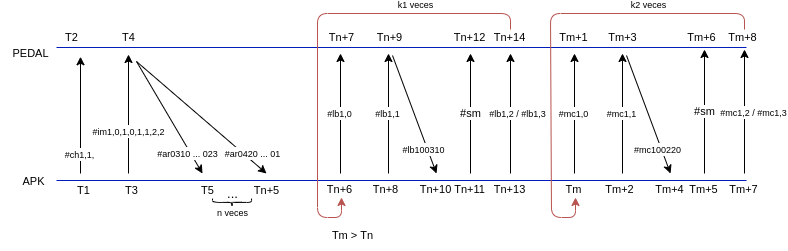
\includegraphics[scale=0.58]{images/diagram-protocol-in-calibration.png}
        \caption{Protocol de comunicación en la calibración}
        \label{fig: diagram-protocol-in-calibration}
    \end{figure}

    \subthesischapter{Implementación de la interfaz gráfica para la representación de datos EMG}
    En el contexto del desarrollo de la interfaz de calibración clínica para la rehabilitación neuromuscular de pacientes con enfermedades cerebrovasculares
    fue necesario la implementación de la clase \underline{CoordinateSystem}. Esta clase, diseñada para extender \textbf{VisualElement}\footnote{Es un elemento visual de Unity3D } en Unity, representa el núcleo de la representación 
    gráfica de los datos EMG en la aplicación móvil. Uno de los aspectos clave de esta implementación 
    radica en su capacidad para generar un sistema de coordenadas dinámico y animado que se ajusta a las variaciones en los datos recibidos.

    \vspace{10pt}
    En el constructor de la clase \underline{CoordinateSystem}, se establece la estructura básica del sistema de coordenadas. Se crean y configuran elementos visuales esenciales, como el 
    marco (frame), los ejes (axes), la ventana de visualización (window), y las etiquetas de los ejes x e y (xAxisLabel y yAxisLabel). Para proporcionar contexto a los datos 
    representados, se han desarrollado métodos para agregar etiquetas a los ejes x e y. Estas etiquetas, definidas como objetos Label, muestran los 
    valores correspondientes a las coordenadas en el sistema. La inclusión de estas etiquetas es esencial para que los profesionales de la salud y los pacientes 
    comprendan el significado de los datos EMG presentados, mejorando así la utilidad clínica de la interfaz. 
    
    \vspace{5pt}
    Estos elementos son fundamentales para la presentación adecuada de los datos EMG en el contexto clínico, pero además, se aplican estilos \textbf{USS}\footnote{Son archivos de texto inspirados en las hojas de estilo en cascada (CSS) de HTML} a estos, definidos en archivos específicos (SystemCoordinateUSS.uss), para asegurar una 
    presentación visual coherente y atractiva, ver figura \ref{fig: graph-emg}.

    \begin{figure}[ht]
        \centering
        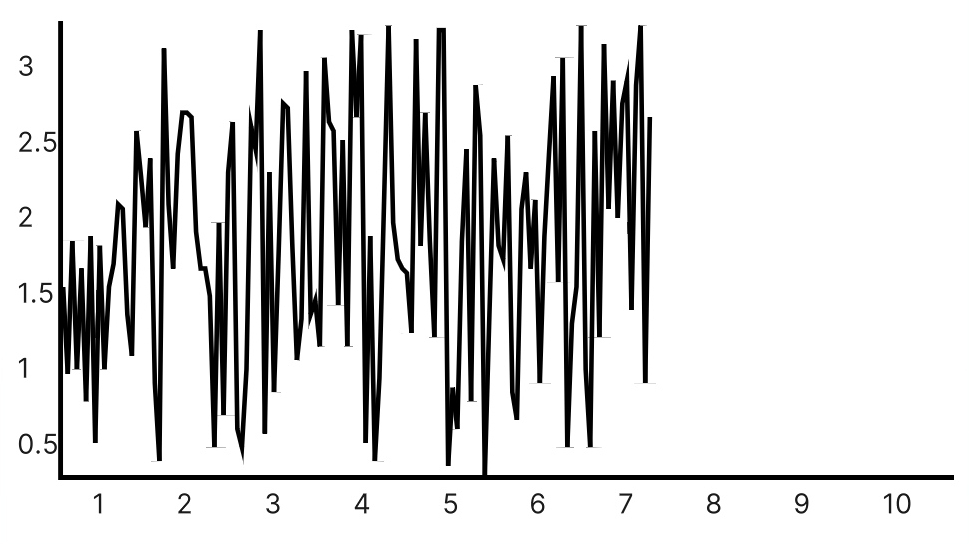
\includegraphics[scale=0.25]{images/emg-graph.jpg}
        \caption{Gráfico de representación de datos EMG}
        \label{fig: graph-emg}
    \end{figure}

    \vspace{10pt}
    Adicional a lo anteriormente mencionado la clase proporciona métodos para trazar puntos y funciones en el sistema de coordenadas. A través de los métodos PlotPoint() y PlotFunction(), la 
    aplicación puede representar los datos EMG de forma gráfica y dinámica. Además, se ha implementado una funcionalidad de animación que permite mostrar la progresión de los datos en el tiempo. El método 
    DrawFunction() utiliza técnicas de interpolación para crear una animación fluida, mejorando así la comprensión de la obtención de los datos en la línea de tiempo.

    \newpage    
    \subthesischapter{Escenarios de entrenamiento}
    La creación de las escenas es dinámica, pues se adapta a los valores de 
    modalidad y parámetros seleccionados en la configuración del juego. Estos valores son fundamentales, ya que 
    determinan el funcionamiento y por ende la experiencia de juego. Para llevar a cabo dicha tarea, fue necesario implementar un script 
    llamado WorldCreator.cs.

    \vspace{10pt}
    WorldCreator.cs es el núcleo de nuestra creación escénica. Este script se encarga de construir la totalidad del entorno del 
    juego. El método Awake() en el script WorldCreator cumple una función fundamental en la inicialización y preparación del escenario 
    de juego. En primer lugar, verifica la integridad del objeto trackPrefab, asegurándose de que no sea nulo mediante una aserción (Assert).
    Este objeto representa la pista sobre la cual se construirá el mundo del juego. A continuación, se procede a la creación dinámica del terreno 
    (Terrain) del juego. Se genera un nuevo objeto de datos de terreno (TerrainData) y se asigna al terreno recién creado. Además, en el método se 
    calcula y almacena las dimensiones del objeto de la pista (trackPrefab) utilizando el componente MeshFilter. Estas dimensiones 
    se utilizan posteriormente para posicionar los árboles y otros elementos de manera coherente respecto a la pista, garantizando la cohesión visual 
    del mundo del juego. Por último, el método Awake() asigna el material (terrainMaterial) al terreno, definiendo así la apariencia visual del paisaje.
    Este proceso sienta las bases para el entorno tridimensional en el cual se desarrollará la acción del juego.

    \begin{figure}[ht]
        \centering
        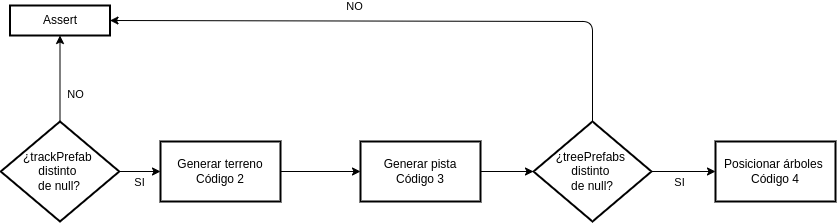
\includegraphics[scale=0.5]{images/generate-world.png}
        \caption{Flujo para la creación del entorno de juego}
        \label{fig: generate-world}
    \end{figure}

% \begin{center}
% \begin{minipage}{0.8\textwidth}
% \begin{lstlisting}[language=c, caption={Generar terreno},label={hola}]
%  //Obtener el terreno activo en la escena
%  terrain = Terrain.activeTerrain;
 
%  // Crear un nuevo objeto de datos del terreno
%  var data = new TerrainData();

%  terrain = Terrain.CreateTerrainGameObject(data).GetComponent<Terrain>();
 
%  // Establecer la posición del terreno en el origen del mundo
%  terrain.transform.position = Vector3.zero;     

%  // Obtener los límites del objeto de pista  mediante su componente MeshFilter           
%  var bounds = trackPrefab.GetComponent<MeshFilter>().sharedMesh.bounds;
%  trackSize = bounds.size;
 
%  // Asignar material al terreno generado
%  terrain.materialTemplate = terrainMaterial;
% \end{lstlisting}
% \end{minipage}  
% \end{center}

% \begin{center}
% \begin{minipage}{0.8\textwidth}
% \begin{lstlisting}[language=c, caption={Generar pista}]
%  float zMin = chunkIndex * chunkSize;
%  float zMax = zMin + chunkSize;
%  terrain.terrainData.size = new Vector3(chunkSize, maxHeight, zMax);

%  var track = Instantiate(
%                  trackPrefab, 
%                  new Vector3(chunkSize*0.5f, 0.0f, zMin), 
%                  Quaternion.identity
%              ).transform;

%  track.localScale = new Vector3(1.0f, 1.0f, chunkSize / trackSize.z);
% \end{lstlisting}
% \end{minipage}  
% \end{center}

% \begin{center}
% \begin{minipage}{0.8\textwidth}
% \begin{lstlisting}[language=c, caption={Posicionar árboles}]    
%  for (int i = 0; i < treeDensity; i++) {
%     float side = Random.value > 0.5f ? 1.0f : 0.0f;

%     // Generar coordenadas aleatorias dentro del rango especificado
%     float z = Random.Range(zMin, zMax);  

%     float x = Random.Range(0, chunkSize * 0.5f - trackSize.x * 0.5f) * side  +
%               Random.Range(chunkSize * 0.5f + trackSize.x * 0.5f, chunkSize) * 
%               (1 - side);

%     float y = terrain.SampleHeight(new Vector3(x, 0, z)); 

%     int treeIndex = Random.Range(0, treePrefabs.Length);
    
%     // Instanciar el árbol en las coordenadas x, y, z 
%     Instantiate(
%         treePrefabs[treeIndex], 
%         new Vector3(x, y, z), 
%         Quaternion.identity
%         );
%  }

%  // Actualizar los cambios en el terreno
%  terrain.Flush();
% \end{lstlisting}
% \end{minipage}  
% \end{center}


    \vspace{10pt}
    %MOVIMIENTO DEL JUGADOR
    Utilizando los datos de velocidad angular ($v_{a}$) capturados a través del sensor óptico del pedal, se lleva a 
    cabo un conjunto de cálculos con el fin de determinar la posición actual del jugador en cada fotograma 
    del juego. Este proceso implica el cálculo de la velocidad lineal ($v_{l}$) a partir de la $v_{a}$, lo 
    cual se logra mediante la aplicación de la ecuación~\ref{eq: dist_calc}, donde r es longitud desde del eje de rotación del pedal hasta el pedal.
    \begin{equation}
        v_{l} = v_{a}r
        \label{eq: dist_calc}        
    \end{equation}
    Ante la disparidad entre la velocidad de recepción de los datos provenientes del pedal, la cual ocurre a una tasa más lenta que la de actualización de los fotograma en Unity
    (ejemplo: 100 ms en comparación con los 16.67 ms necesarios para actualizar los 60 fotogramas por segundo de renderizado en Unity), surge un desafío de sincronización entre la información 
    recibida y los fotogramas de renderizado. Para solucionar este problema, se utilizó la técnica de interpolación, una estrategia que se utiliza para suavizar los movimientos 
    del jugador y lograr una transición más fluida entre los datos recibidos y la representación visual en la pantalla.

    \vspace{10pt}
    % En nuestro caso, fue posible estimar la posición del jugador en los fotogramas intermedios entre los datos recibidos usando el siguiente algoritmo:
    Descripción del algoritmo utilizado, ver figura~\ref{fig: interpolation-algorithm} para más detalles:
    \begin{enumerate}
        \item Se utilizan dos variables, \textbf{finalSpeed} e \textbf{initialSpeed}, inicializadas en 0, para determinar la velocidad inicial y final en cada segmento de tiempo de 100 ms.
        \item En el método \textbf{Update()}\footnote{Es una función especial en Unity que es llamada en cada script, durante cada frame.}, se emplea la técnica de interpolación para calcular 
        una velocidad suavizada, basada en las velocidades almacenadas previamente. Ver código \ref{code: interpolation}
    \end{enumerate} 

    \begin{figure}[ht]
        \centering
        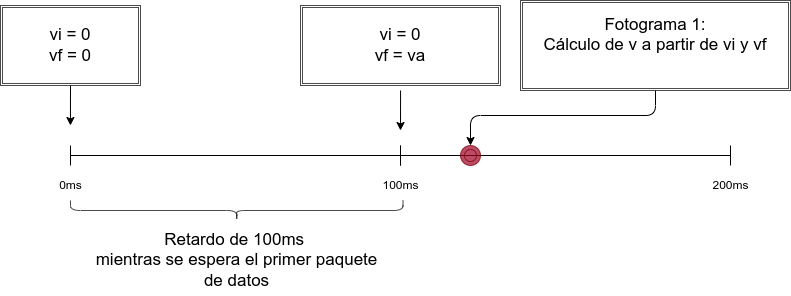
\includegraphics[scale=0.4]{images/interpolation-algorithm.png}
        \caption{Funcionamiento del algoritmo en los primeros 200ms}
        \label{fig: interpolation-algorithm}
    \end{figure}

\begin{center}
\begin{minipage}{0.8\textwidth}
\begin{lstlisting}[language=c, label={code: interpolation}, caption={Controlador de movimiento}]
delta += Time.deltaTime;
 
if(delta > 0.001f) {
    delta = 0;
    finalSpeed = newSpeed;
    initialSpeed = finalSpeed;
}

currentSpeed = Mathf.Lerp( 
    initialSpeed, 
    finalSpeed, 
    delta
);

transform.Translate(currentSpeed * Time.deltaTime);
\end{lstlisting}
\end{minipage}
\end{center}


    \subsubthesischapter{Modalidad Ligero}
    La modalidad ligero, basada en el entrenamiento del tren inferior, se presenta como el primer escenario de juego. En esta 
    modalidad, los parámetros de distancia o tiempo, seleccionados en el menú de configuración de la rutina, sirven como los pilares 
    fundamentales del entrenamiento.

    \vspace{10pt}
    La lógica subyacente del juego en dicha modalidad es la siguiente: al inicio, los usuarios establecen el valor de la distancia o el tiempo en el menú de configuración de las rutinas. Estos valores se utilizan como criterios para mejorar las estadísticas del jugador durante el juego. Por ejemplo, si se establece una distancia de 10 metros, el objetivo del jugador será completar esta distancia en el menor tiempo posible. De manera similar, si se elige un tiempo de 3 minutos, el objetivo será recorrer la mayor distancia posible dentro de ese límite temporal.

    \vspace{10pt}
    Para implementar esta lógica, fue necesario crear un terreno virtual que se reconstruye dinámicamente según la posición actual del jugador. Esto asegura que el jugador permanezca dentro del área de juego y evita que se pierda la coherencia del juego. Al finalizar cada rutina de rehabilitación en esta modalidad, las estadísticas del jugador son actualizadas para reflejar su desempeño, lo que proporciona una retroalimentación valiosa para su progreso.

    \subsubthesischapter{Modalidad Clinico}
    La modalidad clínico de nuestro juego serio representa una innovación significativa en nuestra aproximación terapéutica. Además de las características previamente mencionadas, esta modalidad integra los valores de la señal IEMG (Electromiografía de Superficie) capturados por nuestro pedal motorizado. Esta señal se convierte en un componente fundamental para establecer los desafíos en la escena del juego de esta modalidad.

    \vspace{10pt}
    En esta modalidad clínica, se definen tres puntos clave en el recorrido hacia la meta. En cada uno de estos puntos, el juego verifica la media aritmética de los niveles de IEMG capturados. Estos niveles se comparan con los valores de referencia predefinidos que se establecieron durante la fase de calibración y configuración del juego. Si la media de los niveles de IEMG en un punto dado cumple con los requisitos establecidos, el jugador supera el reto asociado a ese punto y avanza en el juego.


     
    \subthesischapter{Generación de reportes estadísticos}
    Con el objetivo de obtener estadísticas precisas y eficientes de las rutinas de entrenamiento, se desarrolla el script StatisticsUIController.cs. 
    Este tiene la responsabilidad de recuperar los datos almacenados en la base de datos y actualizar los valores pertinentes en 
    los gráficos presentados en la figura~\ref{fig: statics-graphs}. Para acceder a detalles específicos del Gráfico 1, el usuario puede 
    seleccionar la barra correspondiente al día deseado. En este caso, se mostrarán el valor promedio %como la desviación estándar 
    de los datos relacionados con la velocidad y la MCV de las rutinas realizadas, ver figura \ref{fig: statics-graphs} c)  .
    
    \begin{figure}[ht]
        \centering
        \subfigure[Gráfico 1]{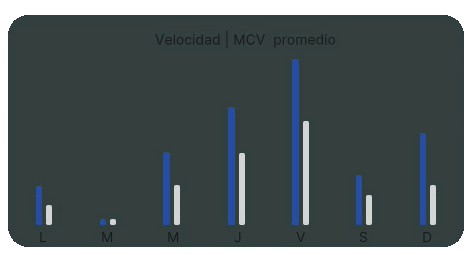
\includegraphics[height=5.2cm, width=0.45\textwidth]{images/ui/ui15-graph1.png}}
        \subfigure[Gráfico 2]{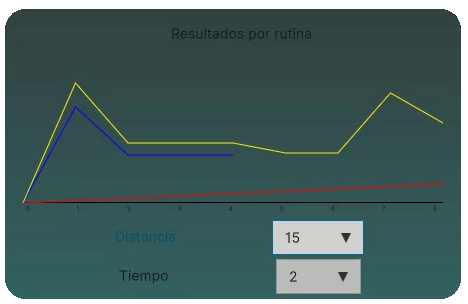
\includegraphics[height=5.1cm, width=0.45\textwidth]{images/ui/ui16-graph2.png}}

        \subfigure[Menú]{
\includegraphics[scale=0.7]{images/ui/ui15-menu.png}}
        \caption{Gráficos estadísticos}
        \label{fig: statics-graphs}
    \end{figure}

    \subsubthesischapter{Generación de los valores del Gráfico 1}
    El primer gráfico figura \ref{fig: statics-graphs} a) permite visualizar los valores promedio de velocidad y MCV
    obtenidos en las rutinas de entrenamiento diarias. Dichos valores se obtuvieron a partir de las ecuaciones \ref{eq: 2}, \ref{eq: 3}.    
    
     \begin{equation}
        V_{i} = \frac{\sum_{j=1}^{k} v_{j}}{k}
        \label{eq: 2}
     \end{equation}
     \begin{equation}
        MCV_{i} = \sum_{c=1}^{4}\frac{\sum_{j=1}^{k} mcv_{c j}}{k}
        \label{eq: 3}
    \end{equation}
    Donde:
    \begin{itemize}
        \item $V_{i} (MCV_{i})$: valor promedio de velocidad(MCV) obtenido el i-esimo día.
        \item $v_{j}(mcv_{cj})$: velocidad(promedio de MCV del canal c) obtenido en la rutina j del i-esimo día. 
        \item $k$: es el número de rutinas ejecutadas el i-esimo día 
    \end{itemize}
    La representación visual de las estadísticas se logró mediante la manipulación de elementos visuales definidos en el archivo de diseño UXML. Utilizando Unity 
    UIElements, se crearon contenedores (VisualElement) para cada día de la semana y se asignaron alturas proporcionales a los resultados promedios obtenidos. Los 
    elementos visuales se actualizan dinámicamente a través del script StatisticsUIController.cs.

    \subsubthesischapter{Generación de los valores del Gráfico 2}
    El segundo gráfico figura \ref{fig: statics-graphs} b) permite visualizar los valores de velocidad, distancia y tiempo 
    correspondientes a cada rutina de entrenamiento ejecutada. Para ello, se utilizan datos provenientes de las entidades 
    de la base de datos, específicamente, de DoEntity y RutineEntity. Estos datos se procesan y se organizan 
    en una representación gráfica compuesta por tres curvas representadas por dichas magnitudes y generadas a partir de la clase 
    SystemCoordinate, donde la coordenada \textbf{x} representa el índice de la rutina \textbf{y} la coordenada y representa la magnitud correspondiente (distancia, tiempo o velocidad). Estas curvas 
    se visualizan sobre un elemento VisualElement de Unity3D, proporcionando así una representación gráfica clara y comprensible del 
    comportamiento de los datos asociados a cada rutina de entrenamiento ejecutada.
    

    \subsubthesischapter{Persistencia de los resultados estadísticos}
    En la fase final del juego, se implementó un código crucial para capturar y guardar los resultados obtenidos en la rutina de entrenamiento. Utilizando la clase DateTime de las bibliotecas de c\#, 
    se registra la fecha y la hora exactas del final del juego. Estos datos se almacenaron en una estructura adecuada y se insertaron en la base de datos correspondiente. La clase CibiofibDb facilitó esta 
    operación al proporcionar métodos para añadir datos (addData()) y cerrar la conexión con la base de datos (close()). Este proceso garantizó la persistencia de los resultados en la tabla Do, lo que 
    permite un análisis detallado del entrenamiento en la sesión de \textbf{Estadísticas}.


    % \textbf{Configuración del entrenamiento} \\ 
    % ----- menu de parámetros ----------

    \subthesischapter{Conclusiones del capítulo}
    Se presentó una descripción del sistema de adquisición de datos para rehabilitación, sus componentes,
    características distintivas y su funcionamiento. Se identificaron y definieron los requisitos del juego 
    serio, tanto funcionales como no funcionales, así como los actores y casos de usos del sistema que establecieron 
    las bases fundamentales para el desarrollo de la aplicación. Se realizó un minucioso diseño de la base de datos, 
    abarcando tanto el modelo lógico como el físico, lo que aseguró una estructura robusta y eficiente para el 
    almacenamiento de los datos. La manipulación de los datos se abordó de manera integral, desde la conexión con 
    la base de datos hasta la persistencia de los resultados estadísticos. Se diseñó e implementó la comunicación
    con el pedal motorizado y la implementación de la interfaz gráfica para la representación de los datos EMG. 
    Se definieron los escenarios de entrenamiento para las modalidades Ligero y Clínico, asegurando 
    una cobertura completa de las necesidad de entrenamiento del usuario. Por último en el ámbito estadístico se desarrolló 
    una serie de gráficos para el seguimiento de los resultados en las rutinas de entrenamiento.   
    

\end{thesischapter}